\documentclass[oneside, twocolumn]{uhphysreport} 

\usepackage{lipsum} 
\usepackage{amsmath}
\usepackage{gensymb}
\usepackage{graphicx}
\usepackage{booktabs}
\usepackage{float} % For forcing table placement

\DeclareMathOperator{\sinc}{sinc}



\title{Grating spectrometer}
\course{Experimental Techniques}
\acyear{2023 - 2024}
\major{$\mathit{1^{e}}$ bachelor FYS}
\date{\today}


\author{Tibe Cornelis (2470582) \\ Thomas Reynders (2467872)}
\begin{document}

\maketitle

\thispagestyle{fancy}
\numberlesssection{Summary}

This experiment focuses on deriving the diffraction and point spread function (PSF) properties of a mercury lamp shining light through a grating. The analysis utilizes the Fourier transform and delta function to approximate the slits of the grating.

Derived Data
\begin{itemize}
    \item Transfer functions
    \item Theoretical derivation of wavelengths
    \item Image resolution
\end{itemize}


\cleardoublepage
\tableofcontents
\clearpage

\section{Introduction}
By examining the diffraction patterns of a light source, valuable insights into its spectral composition can be obtained. This lab report focuses on the principles and applications of diffraction gratings, which separate light into its constituent wavelengths through interference.

The experiment uses a grating spectroscope to analyze the emission spectrum of a mercury (Hg) lamp, highlighting key features such as spectral resolution, intensity distributions, and wavelength measurement. These principles are crucial in various scientific fields, from material analysis to astrophysics, where accurate wavelength determination is essential. This experiment emphasizes the practical application of theoretical concepts to observe and quantify spectral phenomena.

\section{Theory}
    Every light source has its own emission spectrum. (A spectrum of the light frequencies that the object emits.)
\newline
    Each of these frequencies has a wave length. When these "collection of waves" called a wave front meets a slit with a width smaller than the wave length, it diffracts.
\newline
    The excact angle of diffraction depends on the frequency of the light wave.
\newline
    By measuring the angle difference, we can obtain knowledge of the exact frequency that was emitted.
\newline
\newline
    When light has passed through a slit of a width comparable to or smaller than the wave length, it diffracts completely, causing the slit to appear as a point light source emitting spherical light waves.
\newline
\newline
    Interfering light waves (waves that meet each other) will interfere with each other. This causes constructive or deconstructive interference depending on whether or not the waves are in phase at the moment of interference. 
\newline    
    Since the phase of the wave changes as the waves travel through space when 2 waves have traveled an equal amount of distance (and they are of the same frequency), they will be in phase.
\newline
    At the angle of diffraction, all waves will therefore approximately be in phase and cause constructive interference.
\newline
    Slight deviations of this angle will cause some waves to have traveled a longer distance, hence being out of phase, causing a dimmer image.
\newline
    A formalization of the dimming of the image is called the point-spread function, where a point, like a light source, seems to have been blurred, increasing its width and height.
\newline
    The same concept explains why 2 objects of smaller size than the point spread function, who are situated close to each other seem to overlap on an image, since their point spread functions overlap.
\newline
\newline
    We will use the Rayleigh criterion to determine the resolution of our image.


    

    
    



\section{Experimental Setup}

    When the mercury lamp reaches its operating temperature, it emits a mixture of spectral lines that appear bluish-white. This serves as the light source for the experiment.
\newline
    The emitted light first passes through a collimator (of width B), producing a more parallel beam before it encounters the diffraction grating. The grating consists of thousands of tiny slits (each with width b and separated by a distance d). As light passes through these slits, it is diffracted, with each frequency corresponding to a specific color. These colors can then be observed through the telescope.
\newline
\newline
    At the zeroth-order position, only plain white light is visible through the telescope. As the telescope is gradually rotated, the field of view briefly becomes completely dark. Continuing the rotation reveals distinct spectral lines arranged according to color. The sequence typically begins with violet, followed by blue, then green, and then two closely spaced yellow lines. Between these bright peaks, fainter spectral lines are visible, including shades of orange.
\newline
    After this sequence has passed through the field of view, the image returns to darkness. Further rotation results in the reappearance of the same sequence of colors, representing the second-order spectrum. The initial sequence corresponded to the first order, whereas subsequent sequences represent higher orders of diffraction.
\newline
\begin{figure} [h]
    \centering
    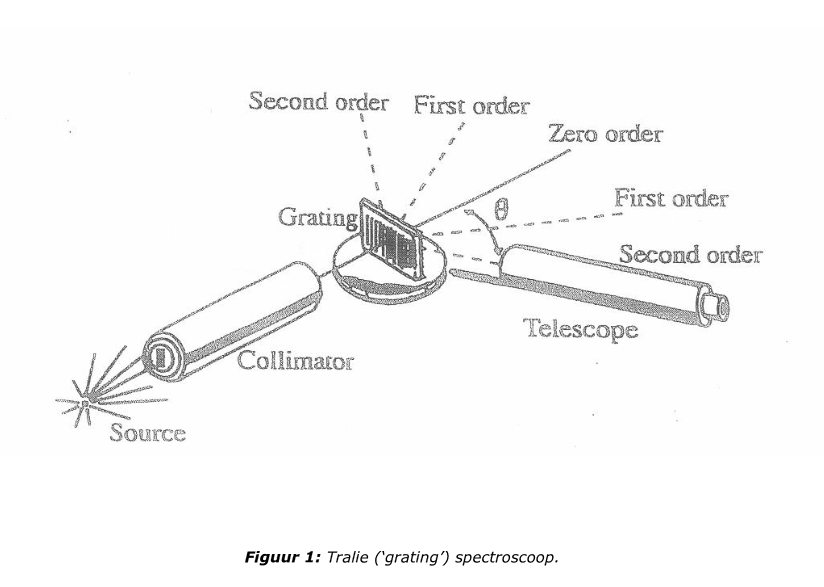
\includegraphics[width=1\linewidth]{afbeelding.png}
    \label{fig:enter-label}
\end{figure}
\clearpage
\section{Results}
    \subsection{Transfer function}
        \subsubsection{For an infinitely wide grating with infinitely narrow \texorpdfstring{$\delta$}{Lg} slits.}
            
            \begin{equation}
                \mathcal{F}[f(x)] = \sum_{n=-\infty}^{\infty} \delta(\omega - 2n\frac{\pi}{d})
            \end{equation}

        \subsubsection{For a finite wide grating with infinitely narrow \texorpdfstring{$\delta$}{Lg} slits.}
            
            \begin{equation}
                \mathcal{F}[f(x)] = \mathcal{F}[Rect(\frac{x}{b})\cdot
                \sum_{n=-\infty}^{\infty} \delta(x-nd)]
            \end{equation}
            
            \begin{equation}
                \mathcal{F}[f(x)] = b \cdot \sinc{ \frac{\omega \cdot b}{2}} * \sum_{n=-\infty}^{\infty} \delta(\omega - 2n\frac{\pi}{d}) 
            \end{equation}
            
        \subsubsection{For a finitely wide grating with a slit of width b}
        
            \begin{equation}
                \mathcal{F}[f(x)] = b \cdot \sinc\left(\frac{\omega b}{2}\right)   \cdot [ \sinc\left(\frac{\omega W}{2}\right) * \sum_{n=-\infty}^{\infty} \delta(\omega - 2n\frac{\pi}{d}) ] 
            \end{equation}
            
   \subsection{Amount of Slits per mm}

        The width of each slit is denoted by \( d \):
        
        \begin{equation}
            d = 1.67 \cdot 10^{-6} \, m
            \label{eq:WidthSlit}
        \end{equation}
        
        The approximate number of slits per millimeter is:

        \begin{equation}
            N \approx 599
            \label{eq:SlitCount}
        \end{equation}
        
    \subsection{Wave length emission lines}
        \subsubsection{Measured angles}
            \begin{table}[H]
                \centering
                \renewcommand{\arraystretch}{1.3}
                \begin{tabular}{l|c}
                    \textbf{Color} & \textbf{Measured Angle (°)} \\
                    \hline
                    Violet & $14.0^\circ$ \\
                    Blue & $15.0^\circ$ \\
                    Green & $17.0^\circ$ \\
                    Yellow 1 & $19.0^\circ$ \\
                    Yellow 2 & $20.2^\circ$ \\
                \end{tabular}
                \caption{Measured angles for different emission lines (First order).}
            \end{table}

            \begin{table}[H]
                \centering
                \begin{tabular}{l|c}
                     \textbf{Color} & \textbf{Measured Angle (°)}\\
                     \hline
                     Violet & $29^\circ$\\
                     Blue & $31^\circ$\\
                     Green & $36^\circ$\\
                     Yellow 1& $41^\circ$\\
                     Yellow 2& $43^\circ$\\
                \end{tabular}
                \caption{Measured angles for different emission lines (Second order).}
                \label{tab:measured_angles_second}
            \end{table}
            
        \subsubsection{Theoretical derivation wave lengths}
        
            Using the formula $\sin{\theta} = \frac{n\lambda}{d}$, under the assumption that the wavelength of violet is known.

            \begin{equation}
                \lambda_{violet} = 404.7\mu m
            \end{equation}

            %Table theoretical derived wave lengths First order
            \begin{table}[H]
                \centering
                \begin{tabular}{c|c}
                     \textbf{Color} & \textbf{Wave length ($nm$)} \\
                     \hline
                     Violet &  404.7\\
                     Blue &  432.2\\
                     Green & 488.3\\
                     Yellow 1 & 543.7\\
                     Yellow 2 & 576.6\\
                \end{tabular}
                \caption{Wave lengths first order}
                \label{tab:wavelengths}
            \end{table}

            %Table theoretical derived wave lengths Second order
            \begin{table}[H]
                \centering
                \begin{tabular}{c|c}
                    \textbf{Color} & \textbf{Wave length ($nm$)} \\
                    \hline
                    Violet &  404.7\\
                    Blue &  432.2\\
                    Green & 488.3\\
                    Yellow 1 & 543.7\\
                    Yellow 2 & 576.6\\
                \end{tabular}
                \caption{Wave lengths second order}
            \end{table}
    \subsection{Resolution}
        Using the Rayleigh criterion, the resolving power is given by.
        
        \begin{equation}
            \mathcal{R} = \frac{\lambda}{\Delta \lambda}
        \end{equation}
        \begin{equation}
            W = \frac{\mathcal{R} \cdot d }{m} = 0.457mm
        \end{equation}
        
        Which is the minimum width of the grating to be able to distinguish 2 waves of length $\lambda_1 = 576.96nm$ and $\lambda_2 = 579.07nm$.
\section{Conclusion}

The experiment successfully demonstrated the principles of diffraction and the practical applications of grating spectroscopes. By analyzing the emission spectrum of a mercury lamp, we measured distinct spectral lines corresponding to different wavelengths, validated through theoretical calculations. The Rayleigh criterion effectively determined the resolving power, highlighting the importance of precise measurement in optical spectroscopy.
\input{Sections/6-Erkenning}


\section*{Appendix: Fourier Transform of the Rectangular Window Function}

\begin{equation}
\text{rect}(a) = 
\begin{cases}
1 & \text{if } |a| \leq \frac{1}{2}, \\
0 & \text{otherwise.}
\end{cases}
\end{equation}

\begin{equation}
F(\omega) = \int_{-\infty}^{\infty} f(t)\, e^{-i \omega t} \, dt.
\end{equation}

Since \( f(t) = 0 \) outside the interval \(\bigl[-\tfrac{\tau}{2}, \tfrac{\tau}{2}\bigr]\), the integral reduces to:
\begin{equation}
F(\omega) 
= \int_{-\frac{\tau}{2}}^{\frac{\tau}{2}} e^{-i \omega t} \, dt.
\end{equation}

Evaluating this integral gives:
\begin{equation}
F(\omega) 
= \left[ \frac{e^{-i \omega t}}{-i \omega} \right]_{-\frac{\tau}{2}}^{\frac{\tau}{2}}
= \frac{1}{-\,i\,\omega} 
\left( e^{-\,i\,\omega \,\frac{\tau}{2}} \;-\; e^{i\,\omega \,\frac{\tau}{2}} \right).
\end{equation}

Using 
\(\sin(\alpha) = \tfrac{1}{2i}\bigl(e^{i\alpha} - e^{-\,i\alpha}\bigr)\), it follows that:
\begin{equation}
F(\omega) 
= \frac{2}{\omega} \,\sin\!\Bigl(\tfrac{\omega \,\tau}{2}\Bigr).
\end{equation}

Expressing this in terms of the \(\mathrm{sinc}\) function yields:
\begin{equation}
F(\omega) 
= \tau \,\mathrm{sinc}\Bigl(\tfrac{\omega\,\tau}{2\pi}\Bigr),
\quad \text{where } 
\mathrm{sinc}(x) = \frac{\sin(\pi x)}{\pi x}.
\end{equation}

\section*{Appendix: Fourier Transform of the Dirac Comb}

Consider the function (sometimes referred to as the "comb function"):
\begin{equation}
f(x) = \sum_{n=-\infty}^{\infty} \delta\bigl(x - n\,d\bigr),
\end{equation}
where \(d\) is the distance between consecutive \(\delta\)-pulses.

The Fourier transform \(F(\omega)\) of a function \(f(x)\) is defined by:
\begin{equation}
F(\omega) 
= \int_{-\infty}^{\infty} f(x)\, e^{-\,i\,\omega\,x}\,dx.
\end{equation}

Substitute \(f(x)\) into the definition:
\begin{equation}
F(\omega)
= \int_{-\infty}^{\infty} 
\left(\sum_{n=-\infty}^{\infty} \delta\bigl(x - n\,d\bigr)\right) 
e^{-\,i\,\omega\,x} \, dx.
\end{equation}
Under suitable conditions, the sum and the integral may be interchanged:
\begin{equation}
F(\omega)
= \sum_{n=-\infty}^{\infty} 
\int_{-\infty}^{\infty} \delta\bigl(x - n\,d\bigr)\, e^{-\,i\,\omega\,x}\, dx.
\end{equation}

The sifting property of the Dirac delta implies:
\[
\int_{-\infty}^{\infty} \delta\bigl(x - a\bigr)\, g(x)\,dx 
= g(a).
\]
By setting \( a = n\,d \):
\begin{equation}
F(\omega)
= \sum_{n=-\infty}^{\infty} e^{-\,i\,\omega\,n\,d}.
\end{equation}

The expression
\(\sum_{n=-\infty}^{\infty} e^{-\,i\,\omega\,n\,d}\)
is an infinite exponential series and can be rewritten as follows:
\begin{equation}
\sum_{n=-\infty}^{\infty} e^{-\,i\,\omega\,n\,d}
= \frac{2\pi}{d} 
\sum_{k=-\infty}^{\infty} 
\delta\!\Bigl(\omega - \tfrac{2\pi k}{d}\Bigr).
\end{equation}

Hence, the Fourier transform of the Dirac comb is:
\begin{equation}
F(\omega)
= 
\frac{2\pi}{d}
\sum_{k=-\infty}^{\infty} 
\delta\!\Bigl(\omega - \tfrac{2\pi k}{d}\Bigr).
\end{equation}

In summary,
\[
\mathcal{F}\Bigl\{\sum_{n=-\infty}^{\infty} \delta(x - n\,d)\Bigr\}
= 
\frac{2\pi}{d} \sum_{k=-\infty}^{\infty} \delta\!\Bigl(\omega - \tfrac{2\pi k}{d}\Bigr).
\]


\vspace{0.5cm}
\printbibliography[heading=bibintoc,title={Literatuur}]
\cleardoublepage

% \appendix changes the numbering of all following sections to letters to reflect that these are appendices.
\appendix
\input{Sections/Checklist}

\end{document}